%!TEX root = ../main.tex

%%%%%%%%%%%%%%%%%%%%%%%%%%%%%%%
%%%%%%%%%%%%%%%%%%%%%%%%%%%%%%%
\chapter{Methodical Modeling}
\label{chap:methodical-modeling}

\begin{textblock*}{.7\textwidth}(70mm-\offset,25mm-\offset)
        \begin{fquote}[Albert Einstein]
            All models are wrong, but some are useful.
        \end{fquote}
\end{textblock*}

This chapter focusses on the description of thoughts and structures of the implementation in Python.
It is not evolving more than necessary details about the package {\itshape diffpssi}, but trying to comprehensible illustrate the structure of the algorithms theirselves and the necessary bordering interfaces.

%%%%%%%%%%%%%%%%%%%%%%%%%%%%%%%
%%%%%%%%%%%%%%%%%%%%%%%%%%%%%%%
\section{Transformer Equipment Modeling}
\label{sec:transformer-modeling}

This section focusses on the dynamics and model behavior of the transformer itself.
It is split into the modeling of the $\Pi$-model and the tap changer control.
For the last mentioned, there are different control schemes implemented and thus described in the subsequent section.
In the beginning, the software structure of the \textit{diffpssi} extension is roughly described, continuing with a dive into the mathematical relations, and specialities.  

%%%%%%%%%%%%%%%%%%%%%%%%%%%%%%%
\subsection{Software Architecture Design}
\label{sec:modeling-architecture}

The first scope of the \textit{diffpssi} extension is to form a modular and easy to maintain class structure. 
The background is to enable support of adding other types of transformers or connected control circuits.
A conceptual chart of this architecture is shown in \autoref{fig:transformer-architecture}.
It is representing only necessary packages, classes, and attributes for the transformer and its control.

\begin{figure}[htbp!]
        \centering
        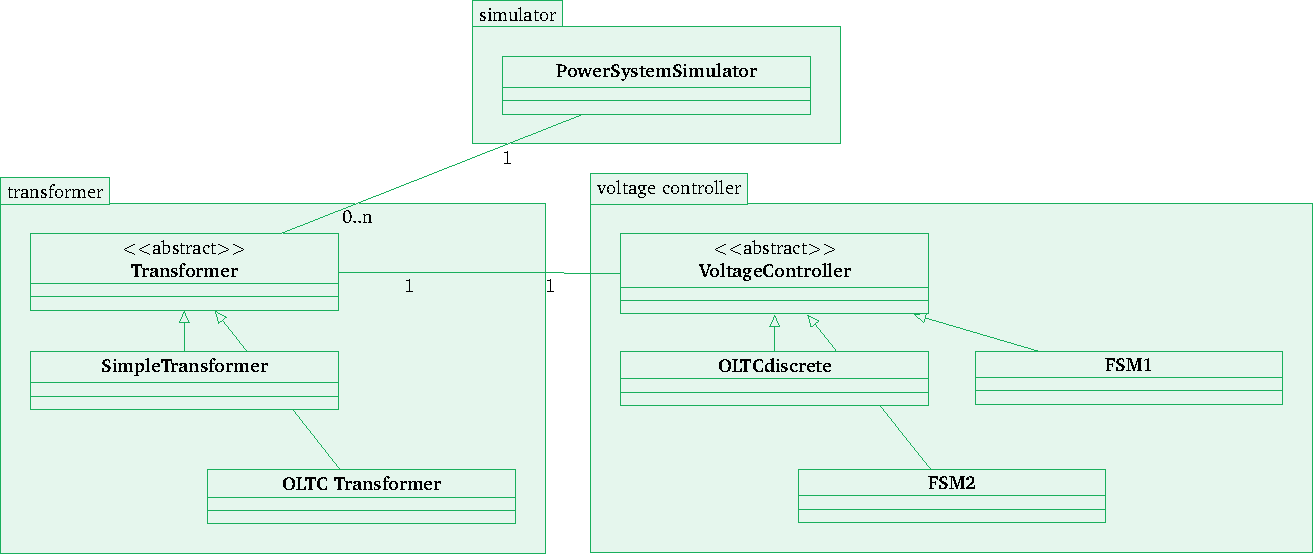
\includegraphics[angle=90, height=18cm]{./tikz_graphics/images/software_structure.pdf}%{modeling/diffpssi_trafo_architecture.png}
        \caption[Architecture of the implemented models in \textit{diffpssi}]{Architecture of the implemented models in \textit{diffpssi}; Using abstract classes for correct interfaces and improved reusability; only necessary packages, modules and classes are depicted.}
        \label{fig:transformer-architecture}
\end{figure}

The main class for the Power System Simulation, hosting the central data structures and results is called \textit{PowerSystemSimulator}.
Models, busbars, lines, but also transformer objects are connected to each other, and on top of that referenced in the main simulation object as groups represented by lists.
The transformers shall be connected in the same way as before, but differing from the initially available transformer model considering just the serial impedance, a simple non-tapping transformer shall be integrated next to a longitudinal tap-changing one.
The room for possible extension, meaning phase shifters or mixtures of these models can be kept by using an abstract class as interface.
This forces the inheritating classses to override the necessary methods, have at least the mandatory attributes.
Copying existing and functional structures is easier as well.

The transformer itself is just a mathematical representation of the $\Pi$-model, considering a serial impedance and two shunt branches.
Connected control units shall be excluded from this, to ensure modularity as well. 
Therefore a lot of different control tweaks can be easily implemented and tested.
To provide a consistant interface here as well, the abstract class \textit{Voltage$\_$Controller} is used.
Within this thesis implemented are a discrete and a continuous \acs{OLTC} controller, and two discrete \acs{FSM} controllers.
These reference to the standardized control blocks as well, e.g. PT1 or integrating elements.

%%%%%%%%%%%%%%%%%%%%%%%%%%%%%%%
\subsection{Implementing a \texorpdfstring{$\Pi{}$}{}-Representative Circuit with Variable Ratio}

Before detailing in the software side of the implemetation, some mathematical differences are explained.
This results on the one hand from the major differences in the literature, especially between \textcite{machowski_2020} and \textcite{kundur_2022}, resp. \textcite{milano_2010}.
On the other hand, the derivation and contraints for usage are not intuitive or directly obvious.
The use and mathematical description of the variable transformer model in the comparative software \textit{DIgSILENT PowerFactory} is hence described in its technical reference manual. 

%%%%%%%%%%%%%%%%%%%%%%%%%%%%%%%
\subsubsection{Mathematical Description and Definitions}

\sidenote{Important definitions and literature differences}
Firstly it is important to comment on the use of indices in this thesis, and especially within the following chapter.
The index 1 is always referring to the \acs{LV} side, the index 2 to the \acs{HV} side. 
The impedances can be concentrated and related to either the \acs{LV}, or as usual to the \acs{HV} side of the transformer. 
The in \autoref{sec:trafo-model} used derivation is using a relation on the \acs{HV} side.
The same accounts for the definition of the \acs{OLTC} ratio $\underline{\vartheta}$.     
The \acs{OLTC} ratio $\underline{\vartheta}$ in this thesis is always placed on the \acs{HV} side.
% If one wants to place this ratio on the \acs{LV} side, the in this thesis defined ratio has to be used reciprocal.
% For the simulation tool, this is crucial to understand and define correctly in order to acquire correct results.

\sidenote{Definition OLTC ratio}
This thesis focusses on an ideal tap changer model at first, other possible considerations from \autoref{sec:further-considerations} are neglected.
As vector groups are as well not considered, the tap ratio stays solely a rational number.
Like previously mentioned, and consequently described, the ratio $\vartheta$ is then placed on the \acs{HV} side of the transformer, and defined as:
\begin{align}
        \vartheta &= 1 + k \cdot \Delta v \label{eq:tap-ratio-hv} \\[6pt]
        \text{with } k &\in [k_\mathrm{min};k_\mathrm{max}]; k_\mathrm{min} \equiv  -k_\mathrm{max} \notag %\label{eq:tap-pos}
\end{align}
Within this definition, $k_\mathrm{min}$ defines the minimum tap position, $k_\mathrm{max}$ the maximum \acs{OLTC} position. 
The variable $\Delta v$ defines the change of the ratio in percent for alterning one position.

\subsubsection{Mathematical Different Representations}

The admittance matrix can be calculated through different ways.
Looking into standard literature and surrounding papers around this thesis, it can be devided in two categories.
Derived from either \textcite{machowski_2020}, versus \textcite{kundur_2022}, \textcite{milano_2010}, or \textcite{burlakin_2024}.
The main difference is, that the placement of the ratio, and the relation of the voltages is on the same side after \textcite{machowski_2020}, and on opposite sides for the others like \textcite{burlakin_2024}.
% When one wants to relate the the tap ratio to the \acs{LV} side, the indices of the admittance matrix have to be changed as before described.
When one would use the admittance matrix after the definition of \textcite{machowski_2020} as
\begin{align}
        \underline{\mab{Y}}_\mathrm{\Pi,T}&= 
        \begin{bmatrix}
            \underline{Y}_\mathrm{T} & -\underline{\vartheta}\underline{Y}_\mathrm{T} \\
            \underline{\vartheta}^*\underline{Y}_\mathrm{T} & -\underline{\vartheta}^*\underline{\vartheta}\underline{Y}_\mathrm{T}
        \end{bmatrix}, \label{eq:admittance-oltc}
\end{align}
one would have to consider switching the bus indices and using the reciprocal ratio of $\vartheta$ at the same time.
As the bus one in the matrix derivation of \textcite{machowski_2020} is the bus where the ratio $\vartheta$ is placed, and the bus would be considered as the \textit{from$\_$bus} in the simulation.

Another thought or way of representing a transformer with off-nominal ratio is described in \autoref{app:current-injection-model}, where the derivation logic after \textcite{machowski_2020} applies.
There, the asymmetric behavior is not represented through the admittance matrix, as this is kept symmetric. 
The matrix is thus split up in a symmetric static contibution accounted in the system admittance matrix and a variable part, respected through different current injections at each bus. 
\begin{align}
        \vartheta_\mathrm{reciprocal} &= \frac{1}{1 + k \cdot \Delta v} \label{eq:tap-ratio-lv}
\end{align}

\subsubsection{Design and Implementation of Algorithmics}

\sidenote{Necessary methods}
As before described in the general architecture of the extension, interfacial methods and attributes are implemented.
Starting with the necessary methods, which can be devided into expectations from the framework itself, the operational unit type transformer, and the novel consideration as dynamic model.
From the framework itself, mainly the three methods \textit{initialize()}, \textit{enable$\_$parallel$\_$simulation()}, and \textit{get$\_$value()} are included.
All submodels have to be initialized with the preset of the measurement voltage at the bus to be measured. 
This accounts only for the \acs{OLTC} related transformers, all others pass this functionality.
To enable parallel simulations, all attributes have to be set as tensors in the expected format of the simualtions.
This is achieved through multiplying the value with a tensor of the shape $(1, {parallel\_sims})$.
For accessing additional, or partly calculated values of interest in the model, the last method is computed.
Although this is currently also an empty function, it can be extended and called by the recorder function of the simulation framework.

Necessary methods of the transformer unit type are the calculation of the static and dynamic admittance matrix.
As for the transformer, and the current goal of implementation, both methods are identical.
If one would want to implement also an automatic tap position configuration for load flow solving, this would provide the sufficient interface.
In the method \textit{calc$\_$admittance()}, the before described transformer admittance matrix is calculated and inserted into the system admittance matrix at each time step.
In the begining of this method, the current measurement bus voltage is aquired and handed to the output function of the connected voltage controller.
This output function is giving back the transformer ratio dependent on the current bus voltage. 
The transformer ratio is then set as an attribute and the admittance then can be calculated and updated.
As an initial value for performing load flow analysis, this ratio is set to $1$ p.u.

In order to consider this model as dynamic, three methods have to be implemented in the transformer itself: \textit{differential()}, \textit{get$\_$state$\_$vector()}, and \textit{set$\_$state$\_$vector()}.
As the transformer itself is containing no dynamics, but its connected controllers do, these methods solely call the methods in the controllers accordingly.

\sidenote{Necessary attributes}
The necessary attributes of the transformers alowing the functions to work properly are implemented as following.
The admittance matrix is always set as attribute.
This allows for evaluation and mapping through the recorder function.
Every transformer has a name, a resistance, a reactance and a susceptance attribute, as well as the transformer ratio $u$, resp. $u_\mathrm{l}$ for the solely longitudinal part.
For the vector group angle rotation, the attribute \textit{theta} is added.
Additionally, the mandatory system related variables for the system base apparent power, the transformer apparent power, the voltages at both busbars, and the parallel simulations are necessary.
Considering the direction of the transformer in the system, the set of variables declaring the bus name, id, and voltage of the \glqq from\grqq~bus is partly defining the installation.
On top of these, tap side and the measurement bus are completing the clear identification.

\sidenote{Comments on the installation}
Focussing more on the installation direction, following procedure is applied in the calculation of the admittance matrix, as it is handed over to the simulation just as a tensor.
A dictionary would be possible as well, as it would namely declare the tap side and non tap side index and impedance.
As used attributes, the attribute \textit{from$\_$bus} and \textit{tap$\_$side} receive either the flag \textit{hv} or \textit{lv}.
For the later attribute the allocation is in the responsibiliity of the user, the first one is allocated through checking the voltages of the busbars.
If the \textit{from$\_$bus} is the lower value of the voltages, the value \textit{lv} is assigned, and vice versa.
The admittance is then calculated for the base scenario, if the tap side of the transformer is not the \textit{from$\_$bus}.
For this scenario \autoref{eq:admittance-matrix-pi} is used.
If the values match, then the admittance matrix indices are switched, and the admittance matric is set as
\begin{align}
        \underline{\mab{Y}}_\mathrm{\Pi,T}&=\underline{Y}_\mathrm{T} \cdot
        \begin{bmatrix}
                \frac{1}{\underline{\vartheta}\underline{\vartheta}^*} & -\frac{1}{\underline{\vartheta}^*} \\
                -\frac{1}{\underline{\vartheta}} & 1
        \end{bmatrix}. \notag
\end{align}

%%%%%%%%%%%%%%%%%%%%%%%%%%%%%%%
\subsection{Tap Changer Control Modeling}
\label{sec:modeling-tap-changer-control}

\sidenote{General interface structure}
As the tap changers, or voltage controllers for the longitudinal ratio of an \acs{OLTC}, are solely controllers, and therefore can also be dissembled in just control blocks, the necessary methods for integration in the module \textit{diffpssi} are limited.
Therefore the abstract base class, used as an interface class here, is containing the funtions \textit{differential()}, \textit{get$\_$state$\_$vector()}, \textit{set$\_$state$\_$vector()}, and \textit{get$\_$output()} for the control purposes.
Adiitionally, as every other dynamic class, both methods \textit{initialize()} and \textit{enable$\_$parallel$\_$\ simulation()} are included in the same way as described before as well.
In case it is needed, every controller is specifying the function \textit{update$\_$vref()}, to update the reference voltage of the control. 
The only varied standard method is \textit{get$\_$output()}, but additional needed ones are necessary dependent on the controller.
These methods are detailed in the subsequent parts of this subsection.
One important note shall be made before any logics are described, as these procedures for all \acs{OLTC} or \acs{FSM} control schemes are based on the assumption, that the admittance matrix is calculated at every time step.
Using multiple step solvers is thus possible, because the differential functions as only time dependent component are coupled to the solver.
The other algorithmics are decoupled from the solver, and thus protected from multiple calls, and following multiple switching events per time step.

\sidenote{Deadband block}
Before going deeper into the control loops, two basic control blocks are implemented into the framework.
The first one is the realization of a deadband block.
This means that if the input value is smaller than a defined threshold, the output will be zero, otherwise it is returning the input value.
The differential function for this block is not necessary, as it is just reacting on the imput and not building up any dynamics or relations towards previous inputs.
The only necessary concern is the enabling of parallel simulations as well, to stay consistent with data types in the calcualtion.

\sidenote{Integrator block}
The second implementated basic block is an integrator, commonly known as I-block in control engineering.
This block has got relations to previous inputs and therefore a differential function, as well as methods for setting and reading the state vector.
This attribute is a storage for the state in the previous timestep, with the differential the next state can be calucated.
As the method \textit{get$\_$output()} is only called by the models, this is the connection to input variables.
An attribute input is set to the handed over value from that function, enabling the differential to be calculated.
Additionally, the output is set to the current state of the control block times a constant multiplication factor $k_\mathrm{i}$ of the integrator.
This integrator is extended by the possibility to set an limiter, as well to externally reset the state and the input variables of the object.
The differential function for an integrator is the input variable times the time step.
As this multiplication is done in the solver function of \textit{diffpssi}, the return of the differential is solely the input value.
The last part is the initialization process, where the first output of this block has to be set, meaning setting the current initial state as the wished or needed output devided through the multiplication factor $k_\mathrm{i}$.
This first output is then also returned.

\subsubsection{Discrete Control Loop}

\sidenote{General aspects\\and references}
This control method represents the currently most used and thus representative control scheme for \acsp{OLTC}. 
With the mechanic nature of the switching mechanism, the control loop can only access discrete ratios within time frames of around a few seconds. 
Such a discrete control loop is described by \textcite{milano_2011,milano_2010}. 
A scheme of this control loop is shown in \autoref{fig:discrete-control-loop}.
This control loop type is beneficial due to its accurate representability of current \acs{OLTC} abilities. 

\begin{figure}[htbp!]
        \centering
        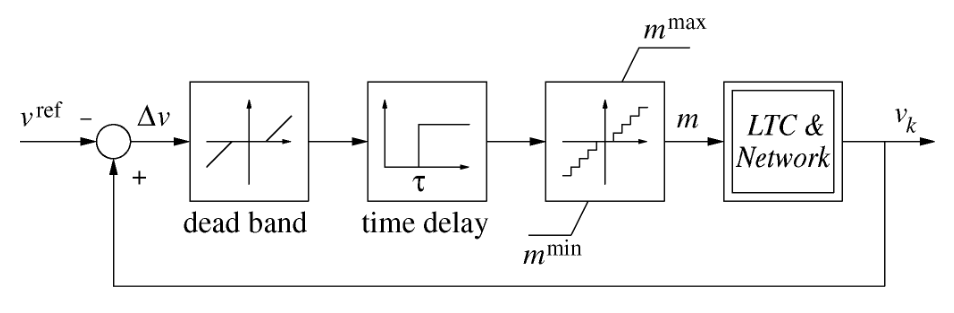
\includegraphics[width=\linewidth]{modeling/oltc_control_scheme.png}
        \caption{Discrete control loop of an \acs{OLTC}; from \textcite{milano_2011}.}
        \label{fig:discrete-control-loop}
\end{figure}

\sidenote{get$\_$output()}
The complete algorithmic scheme is included in \autoref{fig:oltc-program-plan}.
Starting the controller algorithmics as the function input is the voltage measurement at the desired busbar.
As this is physically done in the real world with measurement devices, this value is affected by a time delay the device is taking until the value is passed to the control algorithmics.
The user of this control block can decide, if he wants to consider this in the scheme, by passing a value as float or None to the init function for \textit{pt$\_$1}.

The voltage deviation is calculated, and passed through the deadband filter, after the previous deadband output is stored.
With this, the sign of the voltage difference, or if it is constant, can be checked.
This satisfies the condition, that the tap changer shall be resetted, if the voltage difference is falling below the deadband, or changing signs.
The latter case is indicating an unstable or swinging behavior of the system, where a switch of the tap changer is not helping to stabilize the scenario.

Continuing in the algorithmics, the absolute sign value of the deadband filtered voltage is handed over as argument to the integrator of the time delay.
Either the voltage does not exceed the deadband, so the sign function of numpy is returning zero, or it is exceeding the deadband and the intgrator is incremented with the specified time delay. 
This is happening with no respect if the deviation in voltage is very large or just marginally over the deadband.
At this point one could also think of a variable time delay in this algorithmics.
If the integrator state is now exceeding the time delay attribute of the \acs{OLTC}, a switching operation is triggered with calling the function \textit{switching()} as described in the ongoing.
After the possible switching, the new transformer ratio is calculated and returned to the admittance calculation of the \acs{OLTC}.
Additionally, the integrator block is resetted as switching is completed.

\sidenote{switching()}
The only additional method for the discrete standard \acs{OLTC} scheme is called \textit{switching()}.
Fairly straigth forward it is determing, whether the \acs{OLTC} is in one of its end positions and trying to exceed this end position.
The switching operation is then denied with returning zero as addition to the tap position.
If however an end position is present, but the direction of the switch is resulting in an allowed tap changer position, the switch is passed with either plus or minus one, dependent on the direction of the shift.

\subsubsection{Control Schemes for the Fast Switching module}

The complete algorithmics is strongly oriented on the before described control loop from \autoref{sec:fsm-description} and the to this section connected literature \autocite{burlakin_2024,burlakin_2024a,maschinenfabrikreinhausengmbh_2023}.
In contrast to the shown ratio plot in \textcite{burlakin_2024}, the ratio is not limited by a maximum or minimum.
The only limitation is comming from the maximum tap positions.
This is done because it is more simple to implement, more senseful and allows to obtain a wider bandwith in validation and application in this thesis.
The alterations are fairly small, for a better overview this thesis contains a summarizing program chart in \autoref{fig:fsm-program-plan}.
Similar to the before described discrete \acs{OLTC} scheme, this controller has a \textit{get$\_$output()} method as main, a \textit{switching()} method for both parts, the standard \acs{OLTC} and the \acs{FSM}, and in this case an added funtion for determing the taps to be skipped by the \acs{FSM}.
These methods are subsequently described.

\sidenote{get$\_$output()}
The PT1 described measurement filter is implemented in these controllers the same way at the beginning.
The voltage difference calculation and deadband filtering is applied as well.
The enabling variables are calculated through the numpy sign method and given to the integrators controllers as respective argument.
After that, the taps to be skipped for the \acs{FSM} are calculated.
The switching and resetting for each compartment is triggered, if the respective integrator is exceeding the values of the corresponding time delay constant.
At least the transformer ratio is calculated and returned.

\sidenote{tap$\_$skips()}
The main differing function in the controller classes for the \acs{FSM} is the function \textit{tap$\_$skips()}.
It is simply just the external computation of \autoref{eq:tap-skip} and \autoref{eq:gamma} in one simplification.
In the following section an alternative version is described, but implemented in the same logic and at this point of the algorithm.

\sidenote{switching$\_$k()}
Switching the \acs{OLTC} is equivalent to the switching in the discrete standard \acs{OLTC} scheme.
If this is triggered, the function is approving not trying to exceed the possible tap positions with a switch.
The tap position $k$ then is adjusted either by plus or minus one.
If the \acs{OLTC} is already in an end position, nothing is changed.

\sidenote{switching$\_$m()}
The switching method for the \acs{FSM} is a bit different, concerning the possible skip of taps.
Previously calculated tap skips are an input argument for this function.
Depending on the voltage difference, the switching direction is defined.
After that, the routine checks, if an addition of the tap skips is exceeding the possible tap positions for the \acs{FSM} in a similar way as for the \acs{OLTC}.
If the tap skip is zero, then the voltage difference is too low.
For the possible case of an addition, the tap skips are added to the current tap position $m$ and it is saved subsequently.
If the tap skips are exceeding the range, the according end position is selected as new \acs{FSM} position. 

\sidenote{Differences of\\implementation variations}
Two different versions are implemented, as the in the papers described one \autocite{burlakin_2024,burlakin_2024a} does not match the in the comparison tool \textit{DIgSILENT PowerFactory} available one.
As differences can be described as preferring the \acs{FSM} in the papers, versus the activation of the \acs{OLTC} or the \acs{FSM} is dependent on the voltage difference and the corresponding tap skipping function.
The change from the before detailed implentation for the latter behavior is comparatively small.
The simultaneously allocation of both enabling variables has to be removed, as only the \acs{FSM} one has to be triggered in the first place.
Only if the \acs{FSM} is in one of its end positions, the \acs{OLTC} is getting enabled.
For comparative purposes, both are implemented as seperate voltage controller classes in \textit{diffpssi}.

\subsubsection{Characterization of the Implemented Control Schemes}
% \sidenote{Characterization\\and validation}

For characterization of the control output, two different approaches are selected.
First, a step function is applied, for a maximum gradient inspection.
Further, a continuous function is selected, incrementing the voltage difference on the control loop.
This could be exponential, exponential decaying, or linear increasing.
As the tap changer has maximum positions, and therefore also an operational band, the exponential decaying function is selected as second characterizing input following \autoref{eq:control-characteristic-input}.
\begin{align}
        i(t) &=b - (b-1) \cdot \exp(-a \cdot t) \label{eq:control-characteristic-input} \\[6pt]
        \text{with } a&=0.1,~b=1.1 \notag
\end{align}

\begin{figure}[htbp!]
        \centering
        \begin{subfigure}[b]{.49\linewidth}
                \centering
                \includegraphics[width=\linewidth]{development_files/validation/data/oltc_control_characterization.pdf}
                \subcaption{Continuous Input}
        \end{subfigure}
        \begin{subfigure}[b]{.49\linewidth}
                \centering
                \includegraphics[width=\linewidth]{development_files/validation/data/oltc_control_characterization_jump.pdf}
                \subcaption{Jump Input}
        \end{subfigure}
        \caption[Characterization of the OLTC control loops]{Characterization of the OLTC control loop for a) a continuous input and b) a step input; the input function simulates the to be regulated voltage, the output functions are characterized by $o(t)=i(t) \cdot \underline{\vartheta}_\mathrm{trafo}$.}
        \label{fig:oltc-control-characterization}
\end{figure}

The shown characterizations are the result from multiplying the input function with the controller output and feed back in the control block with the next time input.
This procedure is similar as one would calculate a simple control engineering feedback loop, according to following function:
\begin{align}
        o(t)=i(t) \cdot \vartheta_\mathrm{trafo} \quad\quad \text{for }\vartheta \in \mathbb{Z}. \notag
\end{align}

One important observation can be drawn here.
For the step input reaction in \autoref{fig:oltc-control-characterization} b), the curves of the \acs{FSM} preferred and the voltage dependent control loop are congruent.
The switching occurs approx. $0.2$ s after the step to $1.1$ p.u. input signal, and resulting in a tap position below the \acs{FSM} deadband $0.025$ p.u.
The discrete \acs{OLTC} shows a more delayed response, and just switching until the response is falling under its deadband of $0.05$ p.u.
In the continous increase of the voltage in \autoref{fig:oltc-control-characterization} a) similar characteristics are obtainable.
The major difference here is the earlier switching of the \acs{OLTC} in the voltage dependent control \textit{FSM model 2}.
As the tap skiping function is returning a non-zero value later as the time constant of the \acs{OLTC} is exceeded, switching of the \acs{OLTC} is triggered earlier as well.
Very clearly visible is also the magnitude of one \acs{FSM} switch compared to the \acs{OLTC}, as is is expected to be roughly twice as big.
These behaviors were expected in that ways and intended with the different control models.

%%%%%%%%%%%%%%%%%%%%%%%%%%%%%%%
%%%%%%%%%%%%%%%%%%%%%%%%%%%%%%%
\section{Application of Voltage Stability}
\label{sec:application-voltage-stability}

As previously discussed in \autoref{sec:voltage-stability} concerning voltage stability, ensuring power quality is a secondary goal.
Concerning that voltage stability, regardless of short- or long-time evaluation, is a topic of power quality, it is hard to determine a stable or instable operation point.
In terms of static possible solutions, there are a lot of tools determing the critical points, as well as the current distance to it.
Looking into the short-term, more dynamic assessment, there are less elegant solutions. 
This thesis is trying to keep the perspective on both, short- and long term voltage stability.
The following is the approach to synthesize a toolset for voltage stability analysis, that is at least dynamically comparable.
As Nose Curves are a valid and popular tool, they shall be implemented first. 
Afterwards the time series calculation is tried to be integrated in this static evaluation, including tap changer dependent behavior.
Lastly, a more dynamic rating of a scenario shall be computed, enabling also the confirmity with grid codes for example.

%%%%%%%%%%%%%%%%%%%%%%%%%%%%%%%
\subsection{Generation of Nose Curves}
\label{sec:nose-curves}

This section describes the implementation of a prevoiusly discussed static voltage analysis tool.
The generation of Nose Curves helps in finding the critical loading of the system at the bus of interest, although it is static nature. 

\subsubsection{Basic Simplification Idea}

\textcite{ajjarapu_1992, ajjarapu_2007} are presenting a method for numerical calculation of nose curves in their work. 
It is called {\itshape Continuation Power Flow} and is based on a modified Newton-Raphson method.
The differences rely in a slightly different definition of the power flow equations, considering a load factor $\lambda$.
Combined with a predictor-corrector iterative solver method, this algorithm is capable of nose curve calulation, and finding the critical loading of the system.
While in the first work \autocite{ajjarapu_1992}, only the upper part of the curve including the critical point is calculated, the second work \autocite{ajjarapu_2007} is capable of calculating the complete curve with both solutions. 
As the trade off between implementation effort and the benefits, this method is not exchanging the reduced and simplyfied one.

While this method would be appealing to implement, an additional load flow algorithm, solver, and wrapper seem not profitable for this thesis.
An idea was occuring, just iteratively using the available implemented standard Newton-Raphson algorithm, and implementing a wrapper around it.
The proposed result should be the upper and stable nose curve branch, with the critical point of active power loading.
This shall seem sufficient, as the lower branch solutions are not stable load flow solutions.

The often used parameterization of a function of voltage dependent on the active power and the power angle $\phi$ should be implemented.
In mathematical term, this is expressed as \autoref{eq:pv-mathematical}.
\begin{align}
        \vert \underline{V} \vert : P &\mapsto f(P, \phi) \label{eq:pv-mathematical} \\[6pt]
        Q : \underline{V} &\mapsto f(\underline{V}, \phi) \label{eq:vq-mathematical}
\end{align}
Under consideration of a complex representation of voltage and powers, this algorithm can calculate $V-Q$ curves as well. 
Mathematically this is expressable as \autoref{eq:vq-mathematical}.

\subsubsection{Implementation Details}

\begin{wrapfigure}[12]{r}{0.4\textwidth}
        % \vspace{-20pt}
        \centering
        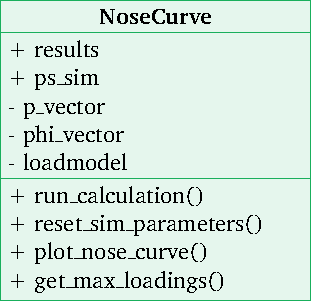
\includegraphics[width=.9\linewidth]{tikz_graphics/images/class_diagram_nosecurve_red.pdf}
        \caption[Class diagram of the NoseCurve class in the package diffpssi]{Class diagram of the NoseCurve class in the package diffpssi.}
        \label{fig:nose-curve-characterization}
\end{wrapfigure}
The implementation of the nose curve generation is realized as a class in the package {\itshape diffpssi.stability$\_$lib.voltage}.
Its class diagram with all attributes and methods is shown in \autoref{fig:nose-curve-characterization}, an extended version is included in \autoref{app:nose-curve}.
For an easy and generic use of the {\itshape diffpssi} package, {\itshape PowerSystemSimulation} objects are used, as well as the function {\itshape do$\_$load$\_$flow()} from the package.

As the before mentioned idea, the method for running the calculation is an iterative wrapper of the load flow calculation. 
This can be as well applied for mutiple busbars as a list input.
At first, the grid and therefore models of the {\itshape PowerSystemSimulation} object has to be cleared with the method {\itshape reset$\_$sim$\_$parameters()}.
Then the active power vector is iterated as load input, together with the power angle $\phi$ for the reactive power in the model.
% Important to note here, is the usage of an {\itshape **kwargs} argument.
The callable for the model is called with load parameters for each load bus as the bus name, and a list with active and reactive power.
The initials of this grid callable are used as the standard values, so only one bus can be varied at a time.
The result is saved as a {\itshape pandas DataFrame} in a \textit{dict}, with the keys being the bus names.

The method {\itshape plot$\_$nose$\_$curve()} is used to plot the results, and is using the {\itshape matplotlib} package.
Further, the method {\itshape get$\_$max$\_$loadings()} can provide details about the critical point.
Giving back a dict with keys as bus names, the values itself are dicts with key of the power angle parameter $\tan \phi$ and the values as {\itshape pandas DataFrame}.
The contained details are maximum active power $P_\mathrm{max}$, the reactive power $Q$ at this point, and the voltage magnitude $\vert \underline{V} \vert$ at the bus.

\sidenote{Parameter variation Nose Curves}
Additionally, the method set \textit{run$\_$variation$\_$calculation()} and its connected automated plotting method \textit{plot$\_$nose$\_$curve$\_$variation()} aims to calculate a nose curve parameter set under variation of a system parameter variation.
This is realized through a callable function, enabling access to the desired object attribute.
Additionally a list of variation values as to be handed over, for iteration over it and saving the result to a dictionary.
This dictionary then can be plotted or accessed over the object as attribute.
The \acs{OLTC} tap dependent Nose Curves from \autoref{fig:oltc-nose-curve} are generated by this functionality

\subsubsection{Results of the Nose Curve Generation}

The following \autoref{fig:nose-curve-simple-grid} shows the generated nose curve for a simple grid as illustrated in \autoref{fig:single-line-voltage-stability}.
The grid is characterized at Bus 1, with a varying power angle as parameter $\tan \phi$.
The power angle $\tan \phi$ is used to vary the power factor of the load, thus representing different load characteristics, as
\begin{align}
        \tan \phi &= \frac{Q}{P}. \notag %\label{eq:tan-phi} \\[6pt]
\end{align}
Displayed are a few combinations with different load characteristics, leading to a different possible maximum acitve power transfer.
\autoref{fig:nose-curve-simple-comp} shows the comparison between the analytical calculation and the implemented solution.
The analytical calculation is carryied out in the same way with identical values as in \autoref{sec:analytical-voltage-stability}.
% For this specific example, the complete calculation, including the set of used parameters, is shown in \autoref{app:analytical-nose-curve}.
What seems conspicious is the missing lower part of the curve, meaning the second possible solution when solving the power flow equations.
Although this seems like a major drawback, the resulting curve contains all the necessary parts, where a stable solution can occur \autocite{cutsem_1998}.
The solution is reaching exactly until the critical point of power transfer.
After that, the load flow calculation does not converge anymore and raises an error.
This error is catched and the iterative wrapper for the first power relation stops.

\begin{figure}[htbp!]
        \centering
        \includegraphics[width=\linewidth]{development_files/theoretical/plots/simple_load_B1_nose_curve.pdf}
        \caption[Examplary generated nose curve for a simple generator - load grid]{Examplary generated nose curves for a simple generator load grid for various power angle level parameters $\tan \phi$; Applied on the grid of \autoref{fig:single-line-voltage-stability} with a characterization at Bus 1.}
        \label{fig:nose-curve-simple-grid}
\end{figure}

\begin{figure}[htbp!]
        \centering
        \includegraphics[width=\linewidth]{development_files/theoretical/plots/simple_load_B1_nose_curve_w-theoretical.pdf}
        \caption[Comparison between the analytical calculation and the implemented solution]{Comparison between the analytical calculation and the implemented solution.}
        \label{fig:nose-curve-simple-comp}
\end{figure}


%%%%%%%%%%%%%%%%%%%%%%%%%%%%%%%
\subsection{Combination of Static Methods with Time Domain Solutions}
\label{sec:comb-time-dimension}

Adding a \acs{TDS} to the static Nose Curve plot is fairly simple and straight forward.
The basic idea is gathering the demanded power by the load as additional recorder function, to overlap the dimensions voltage and power in the static plot.
Additionally using color alteration for the time dimension is keeping the evolvement information as well.
This data is then just added to the plot of Nose Curves.
The backgorund on why this could give a valuable inside, is simply looking into how close to the static solutions of the grid can the system stay under dymanic equalization and control processes.
The static solutions should theoretically match the long-term solutions or states after the equalization processes.
As this dynamic solution is also conditional to the machine and machine controls for example, it could give explanations about missing capabilities from this point, as the nose curves just express the network limits.

Necessary for gathering the missing power information, the method \textit{get$\_$value()} has to be added to the static model \textit{Bus} as well.
There, specifically the apparent power $S$ is calculated through the sum of the models current injections.
With the basic relations
\begin{align}
        \underline{S}&=\underline{V} \cdot \underline{I}^* \notag, \\
        P&=\mathfrak{Re} \{\underline{S}\}\text{, and} \notag \\
        Q&=\mathfrak{Im} \{\underline{S}\} \notag
\end{align}
one can then access the active power as recorder attribute. 
Important to note here is, that the current injection of a simple load cannot be calculated by default, as this model is solely adding a contribution to the admittance matrix of the system.
Therefore this model does not consider current injections.
As proposed workaround, a load attribute \textit{i$\_$inj} is calculated in each iteration of the method \textit{get$\_$admittance()} in the static model \textit{Load} with the relation
\begin{align}
        \underline{I}_\mathrm{inj}=\underline{S}_\mathrm{load}(t) \cdot \frac{\underline{S}_\mathrm{n,sys}}{\underline{V}(t)^*}. \notag
\end{align}

% \commenting{
%         Idea here: Show the dynamic RMS simulation results in the quasi-staionary assessment techniques.
%         These are static solutions to the network, the electromechanic equalization processes should on a long-term watch result in these states.
%         With controls of the machines etc. one can obtain more or less a following of the static solutions until a certain point.
%         If the grid, or the machine, or its control units are stronger, a certain (heavy) level of load increase can be better and faster compensated.

%         Maybe interesting: Can the faster FSM not only increase the time until Voltage envelope is violated, but extend the transferred power as well?        
% }
        
%%%%%%%%%%%%%%%%%%%%%%%%%%%%%%%
\subsection{Using Voltage Envelopes for Criticality Evaluation}
\label{sec:comb-rating-tool}

\begin{figure}[htbp!]
        \centering
        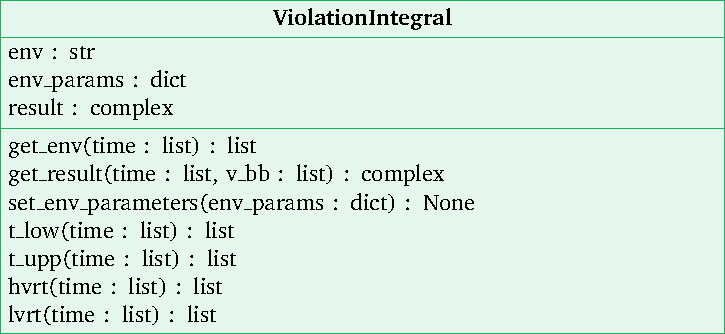
\includegraphics{tikz_graphics/images/class_diagram_violationintegral.pdf}
        \caption[Class diagram for the class ViolationIntegral]{Class diagram for the class ViolationIntegral.}
        \label{fig:class-violation-integral}
\end{figure}

\sidenote{Class\\ViolationIntegral}
The before described method \acs{TVI} from \autoref{sec:stability-indices} is implemented as seperate class \textit{ViolationIntegral} in the package \textit{diffpssi}.
Automated simulations are not considered, as they do not add significant practicability.
Therefore, simply the results vector is just handed over.
The class diagram is displayed in \autoref{fig:class-violation-integral}.

As before described, not only the mathematical describable envelopes are added, but the Machine Type II \acs{FRT} curves when connecting to the medium voltage grids from \autocite{vde-tar_2018,vde-tar_2023} are added as well.
Both envelopes are implemented as a function dependent on the time, giving back a vector in the length of the time vector and being comparable to the bus voltage solution from the power system simulation object.
Envelope parameters can be set with the function \textit{set$\_$env$\_$paramms()}, but can as well be read out through the function \textit{get$\_$env()}.
Here the same logic applies as with the envelope functions before, as a vector with the length of the time vector is given back.

\begin{figure}[htbp!]
        \centering
        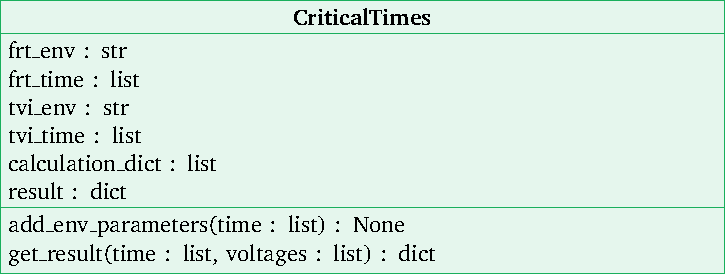
\includegraphics{tikz_graphics/images/class_diagram_criticaltimes.pdf}
        \caption[Class diagram for the class CriticalTimes]{Class diagram for the class CriticalTimes.}
        \label{fig:class-critical-times}
\end{figure}

\sidenote{Class CriticalTimes}
The class \textit{CriticalTimes} is added as well as displayed in \autoref{fig:class-critical-times}.
It is used to enable a calculation of all time steps, where the envelope(s) are violated.
The method accounts just the time stamp, where the envelope is cut from inside to outside, instead of returning all time steps outside of the envelope(s).
The envelopes can be added and results can be calculated through handing over a bus voltage result with time vector.
Results are stored as an attribute as well.
The enevelope functions are re-used from the class \textit{ViolationIntegral}.

%%%%%%%%%%%%%%%%%%%%%%%%%%%%%%%
%%%%%%%%%%%%%%%%%%%%%%%%%%%%%%%
\section{Summary in Short and Simple Terms}

Summarizing this chapter of implementing models and tools, the necessary parts are achieved.
A variable ratio transformer model with its specialities is implemented for non-complex ratios.
The accounting voltage controllers are implemented within a given system allowing for easy access, troubleshooting or extension.
The realization of some extended ideas is described for the modeling of control units.

Regarding the assessment tools for voltage stability, static nose curve calculation is now possible.
This showing the capabilities of the grid, can be extended with a comparative look into the \acs{TDS}, where the difference to the voltage geneartion units can be illustrated.
A quantitative evaluation method between different scenarios is implemented with the \acf{TVI}.
With this, finding critical busbars seems possible as well.